The solution to the problem of redundant work and increased write amplification is query-driven compaction. This 
approach involves writing the valid keys back to the higher levels of the LSM tree.

\subsection{Vanilla Approach}
The flow of range query in vanilla approach is shown in Figure~\ref{fig:vanilla_range_query}. The query runs by 
initiating the iterators for each level of LSM tree and then perform a seek operation on each iterator to find the 
first key that is greater than or equal to the start key of the range query. It then iterates through the
SSTables in the LSM tree and returns the values that fall within the query range. At the end of the range query
execution the state of LSM tree would be same as before the query execution.

\subsection{Query-driven Compaction}
The flow of range query in query-driven compaction is shown in Figure~\ref{fig:query-driven_compaction}. The initial 
setup of level iterators goes the same as in the state-of-the-art LSM range query. Once all the iterators are 
initialized, it performs a seek operation on iterators using the range-query \textit{start key} for each level. The seek 
operation in query-driven compaction performs an extra operation to create partial file flush jobs and adds them to the 
\textit{write queue}. The partial file flush will only happen if the file does not completely overlap with the range-query 
\textit{start key} and \textit{end key}. We can have three scenarios for the partial file flush, which 
are as follows (shown in Figure~\ref{fig:file_range_overlaps}).

\begin{figure*}
    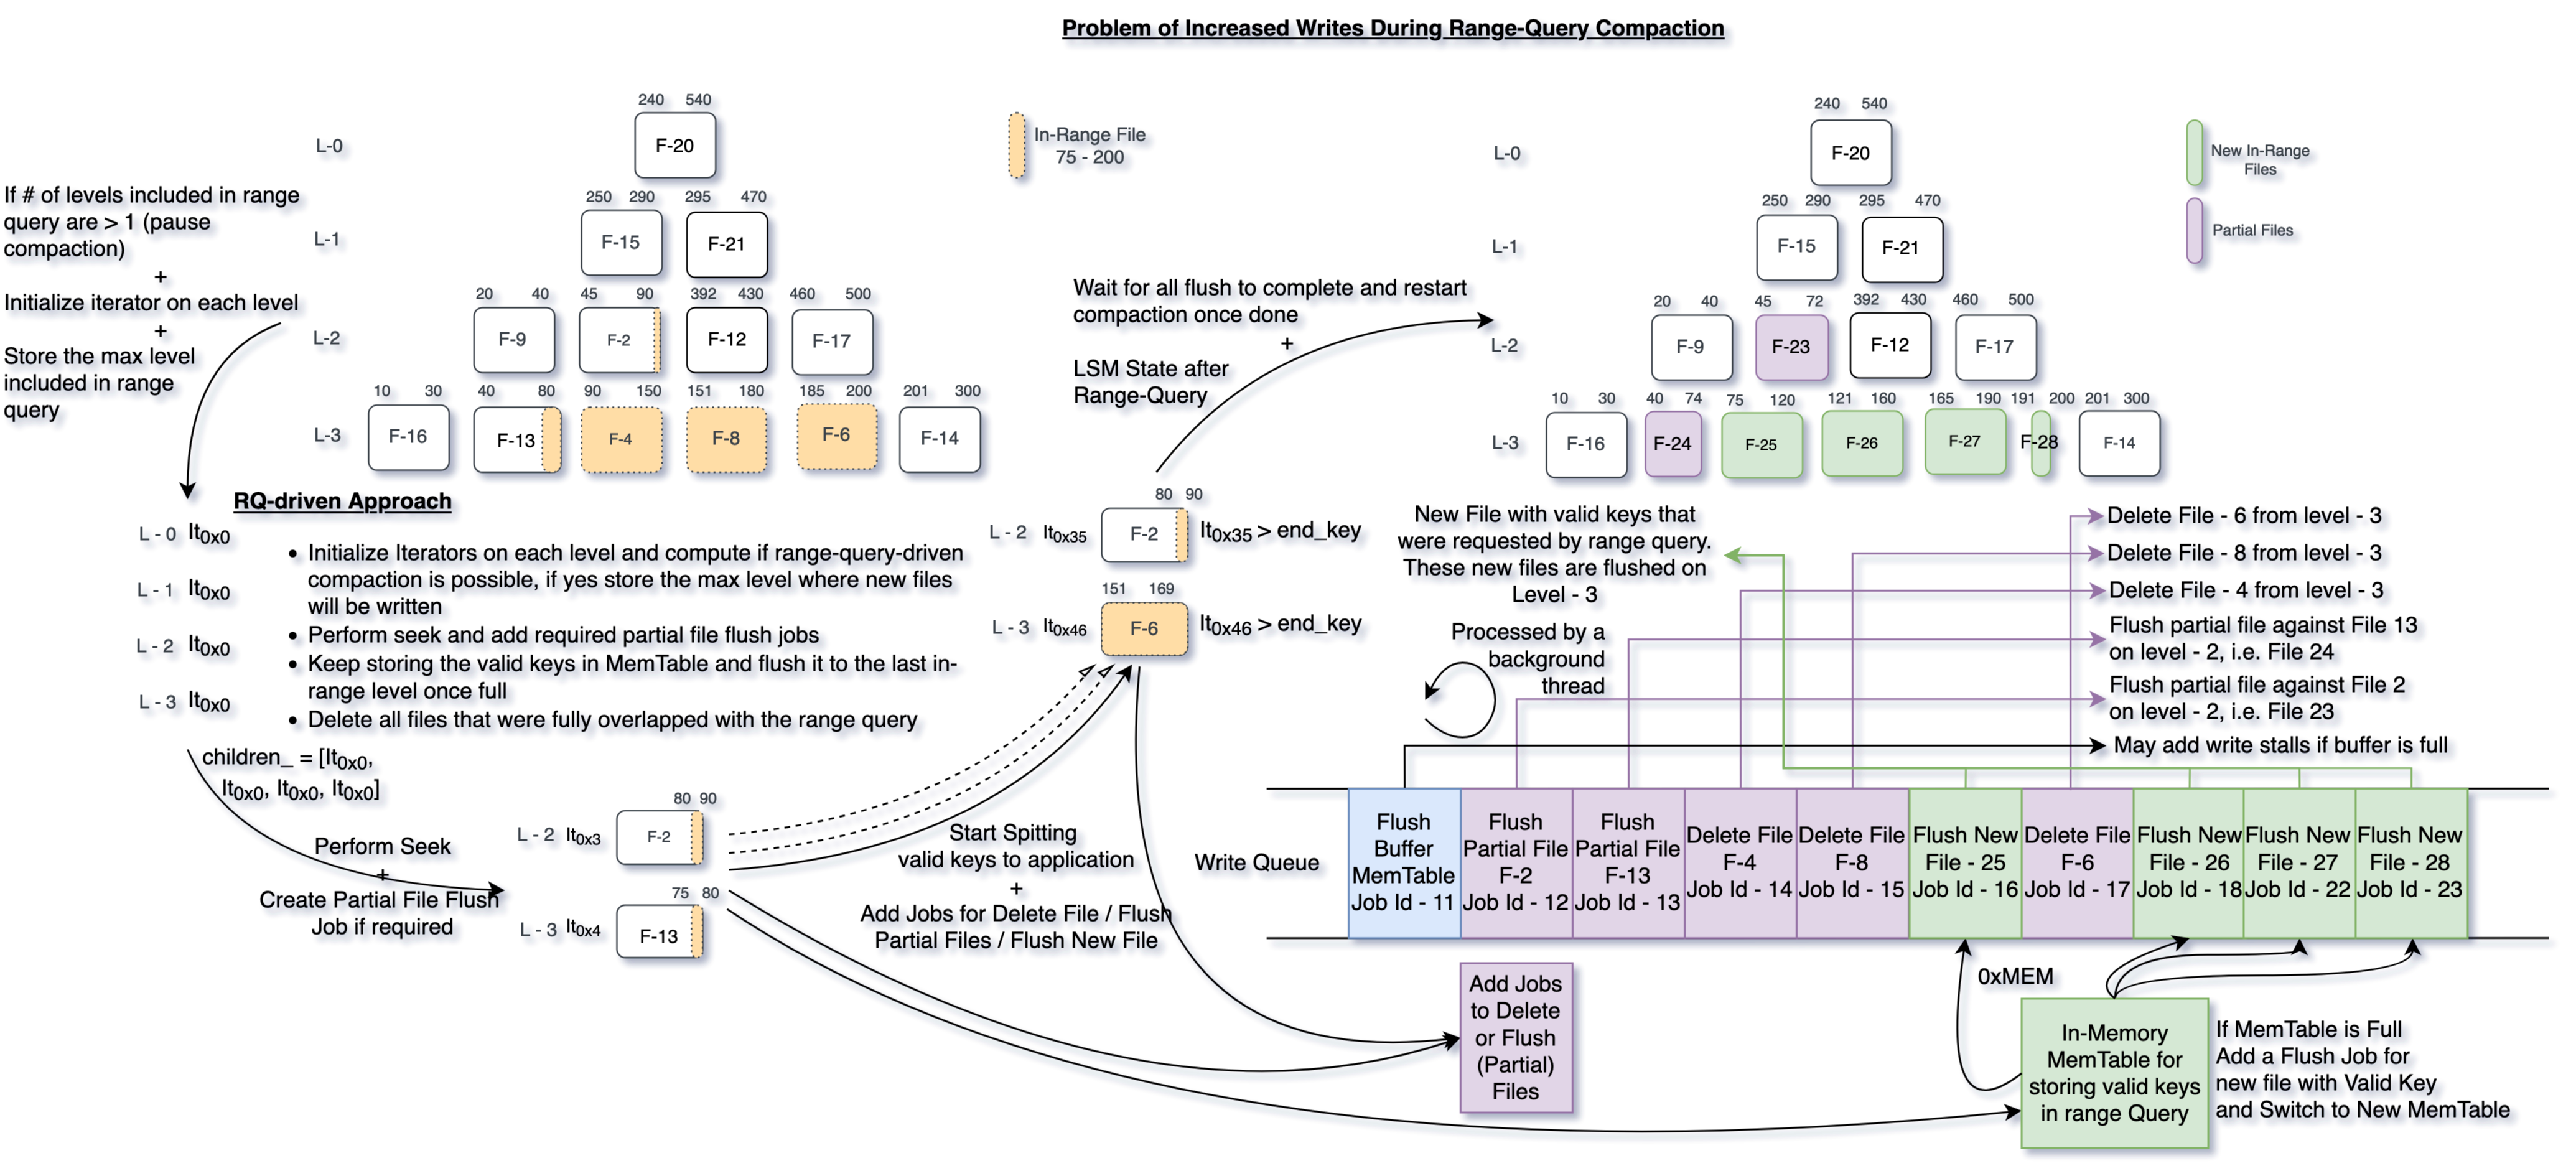
\includegraphics[scale=0.12]{Figures/RQ-driven problem of increased writes.png}
    \caption{Illustration of the problem of increased writes in query-driven compaction caused by reduced overlap. This scenario arises when there is less overlap between levels that are compacted during range query, leading to a higher number of writes.}\label{fig:query-driven_compaction_with_increased_writes}
\end{figure*}

\begin{enumerate}[leftmargin=*,labelindent=0mm, itemsep=0.2\baselineskip]
    \item \textbf{No overlap} In this scenario, the partial file flush will not happen as the file does not overlap. 
    Figure~\ref{fig:file_range_overlaps} (e)
    \item \textbf{Smallest or Largest key overlap \textit{(Partial Flush)}} In this, the smallest or largest key of the 
    file overlaps with the range query start or end key. Figure~\ref{fig:file_range_overlaps} (a) and (b)
    \item \textbf{Head or Tail overlap \textit{(Partial Flush)}} In this, the partial part (having more than one key) 
    overlaps with the range query. Figure~\ref{fig:file_range_overlaps} (c) and (d)
    \item \textbf{The range fits inside file overlap \textit{(Partial-Partial Flush)}} Both the start and end keys of 
    the range query fit completely in the file's smallest and largest keys. Figure~\ref{fig:file_range_overlaps} (f)
\end{enumerate}

These partial flush jobs, that are added to the \textit{write queue} are executed by the background thread, 
parallel to the range query. It flushes the partial part of the file that does not fall in the range query to the same 
level in the LSM tree.

The files that are completely overlapping with the range query \textit{start} and \textit{end key} will be deleted from the lower 
levels and the valid keys will be added to the higher levels in new files. We can have one scenario for the file 
deletion from the lower levels which is as follows.

\begin{enumerate}
    \item \textbf{Complete overlap i.e. \textit{start key} <= smallest key and \textit{end key} >= largest key 
    \textit{(Just Delete)}} All files in the lower level, as well as in higher level, that are completely overlapping 
    with the range query will be deleted by the query-driven compaction. Figure~\ref{fig:file_range_overlaps} (g)
\end{enumerate}
The query-driven compaction also initiates an in-memory buffer of the same size as configured for ingestion buffer to store
and flush the valid keys back to the LSM on higher level. The main thread, that is executing the range 
query will keep on performing the sort-merge operation and returns the valid keys back to the application. Whenever it 
returns a valid key to the application, the query-driven compaction makes a copy and stores it in a specific in-memory 
buffer allocated for it. Once the buffer is full, it creates a new flush job and adds it to the \textit{write queue}. 
Though query-driven compaction does an extra work to remove invalid keys and wirte valid ones back to the LSM, it can 
also add write stalls for few queries to flush all the jobs initiated during this 
operation. This happens because it stops the background work in the start of the range query and wait for all the flush 
jobs to execute successfully at the end of the range query.

Whenever query-driven compaction is triggered during the range query, it will remove all the logically invalid keys and 
tombstones from the LSM tree that fall in that range, which also results in reduced space amplification. This way 
whenever background compactions are triggered after successful query-driven compaction, it will increase the chances of 
trivial moves of files between levels for the minimum overlapping strategy. It will also reduce the write 
amplification for any compaction that has overlapping keys with the previous query-driven compactions.

Keys from Level-0 are not pushed to the last level and there would be no partial flush for the same to 
keep the hot data in lower levels.

\subsection{Informative Compaction}
When the buffers for ingestion are full and additional insert request hits the database, it will keep stalling 
new writes until the buffers are flushed to the disk. The query-driven compaction is beneficial for future queries, but 
it may stall newer writes during the compactions that occur while executing range queries. This necessitates a better 
decision-making strategy to determine whether to proceed with compaction or simply follow the vanilla approach during the 
execution of range queries.

The range query can be diverse, reading one or more files or entries from each level. If the query reads highly overlapping 
keys across multiple levels, the query-driven compaction would remove more invalid keys. However, if the query has only a 
fewer overlapping keys, it may add more overhead of writing valid keys than removing invalid ones.

Once a query-driven compaction is performed, the data for that range will be written into one level. Now, imagine triggering 
a new range query after adding some new keys, assuming that there is some overlap (90\%) with the previous range query, 
and the remaining 10\% is evenly distributed across the entire range. In this scenario, 90\% of the keys will be 
retrieved from the level where the previous query stored valid keys, while the remaining 10\% will be read from other 
levels. If a query-driven compaction is performed, it will result in writing more valid keys at the same level, leading 
to increased writes, as illustrated in Figure~\ref{fig:query-driven_compaction_with_increased_writes}.

% % decision making meta data table %

\begin{table}
    \begin{tabular}{|c|c|c|c|c|}
        \hline
        \textbf{Level} & \textbf{Number of Entries} \\
        \hline
        L-0 & \-- \\
        \hline
        L-1 & \textit{$E_{useful\ 1}$} \\
        \hline
        L-2 & \textit{$E_{useful\ 2}$} \\
        \hline
        L-3 & \textit{$E_{useful\ 3}$} \\
        \hline
        $\vdots$ & $\vdots$ \\
        \hline
    \end{tabular}
    \caption{Number of entries we found in a range [\textit{start\ key}, \textit{end\ key}] for a specific range query from each level}
    \label{table:decision-making-meta-data}
\end{table}

% Decision matrix %
\begin{table}
    \begin{tabular}{ |c|c|c|c|c| }
        \hline
        \hspace*{4.1mm}\textbf{Level}\hspace*{4.1mm} & \hspace*{4.1mm}\textbf{L-1}\hspace*{4.1mm} & \hspace*{4.1mm}\textbf{L-2}\hspace*{4.1mm} & \hspace*{4.1mm}\textbf{L-3}\hspace*{4.1mm} & \hspace*{4mm}$\cdots$\hspace*{4mm} \\
        \hline
        \textbf{L-1} & $True$ & $L_{12}$ & $L_{13}$ & $\cdots$ \\
        \hline
        \textbf{L-2} & $\times$ & $True$ & $L_{23}$ & $\cdots$ \\
        \hline
        \textbf{L-3} &  $\times$ &  $\times$ & $True$ & $\cdots$ \\
        \hline
        $\vdots$ &  $\vdots$ &  $\vdots$ & $\vdots$ & $\ddots$ \\
        \hline
    \end{tabular}
    \caption{Decision matrix generated from Table~\ref{table:decision-making-meta-data}. It helps in choosing consecutive levels for compaction in response to a particular range query. If all are false, it falls back to vanilla}
    \label{table:decision-matrix}
\end{table}

\Paragraph{Solution}
Performing a small amount of work before initiating a range query can aid in making more informed decisions in the 
aforementioned scenarios. Let's assume that every range query has a few \textit{Useful entries} in the LSM-tree that will 
be read from various level\(s\). \textit{Useful entries ($E_{useful}$)} are those that are read from a level to serve the range 
query and can be moved down from lower ($L_i$) level to higher ($L_{i+1..}$) level while eliminating logically invalid entries.
If all the entries from the choosen SST file\(s\) from the lower level does not fall in the range of range query than the remaining entries 
will be written to the same level in smaller (partial) files, as discussed earlier.

Once we have this \textit{Useful entries} data for each level (shown in Table~\ref{table:decision-making-meta-data}), we create a decision matrix, as shown in Table-\ref{table:decision-matrix}. 
In this matrix, each cell corresponds to the boolean value of $L_{[start, end]}$. Here, $L_{[start, end]}$ signifies the 
range of levels where we can initiate the compaction process, extending up to the level where we can conclude the 
compaction for a specific range query. 

When a cell is true, it signifies that the query-driven compaction will use the result of the sort-merge operation for 
levels within the specified range from \textit{start} to \textit{end}, inclusive, and then store it on the \textit{end} level.
There are specific conditions for the truth value of a cell: 
\begin{enumerate}[leftmargin=*,labelindent=0mm, itemsep=0.2\baselineskip]
    \item It is always true on the diagonal of the decision matrix.
    \item It is always false when \textit{end} is less than \textit{start}.
    \item It will only be true when \textit{end} is greater than \textit{start}, and it satisfies below two conditions:
    \begin{enumerate}[leftmargin=*,labelindent=0mm, itemsep=0.2\baselineskip]
        \item The $\frac{E_{useful(end-1)}}{E_{useful(end)}}$ must be in between \textit{lower\_bound} (lb) and 
        \textit{upper\_bound} (ub) thresholds, inclusively.
        \item The cell value at $L_{start, end-1}$ must be true.        
    \end{enumerate}
\end{enumerate}

\begin{flalign}
    \label{eq:full_matrix}
    &L_{[start, end]} =
    \begin{cases}
        \text{False}, & \text{if } \text{end} < \text{start}, \\
        \text{True}, & \text{if } \text{start} = \text{end}, \\
        R_{(start, end)}, & \text{if } \text{end} > \text{start}
    \end{cases} &
\end{flalign}
% where 
\begin{flalign}
    \label{eq:decision_matrix}
    &R_{(start, end)} =
    \begin{cases}
        \text{True}, 
        & \begin{aligned}
            & \text{if } L_{[start, \text{end}-1]} = \text{True}\\
            & \text{ } \land lb \leq \frac{E_{\text{useful(end-1)}}}{E_{\text{useful(end)}}} \leq ub
        \end{aligned}\\
        \text{False}, & \text{otherwise}
    \end{cases} &
\end{flalign}\\

Equation~\eqref{eq:decision_matrix} asserts that \(L_{[start, end]}\) is true only when \(R_{ij}\) is true for all 
\(i\) in the range from \(\text{start}\) to \(\text{end}-1\), where \(j = i+1\). In this context, the 
\textit{lower\_bound (lb)} threshold represents the minimum percentage of entries that should roughly overlap from 
level \(i\) to level \(i+1\) to trigger compaction, and the \textit{upper\_bound (ub)} sets the maximum allowed 
percentage of overlap. If the ratio of overlapping entries falls within the \textit{lower\_bound} and \textit{upper\_bound} 
for all levels from \textit{start} to \textit{end} (\(L_{[start\ end]}\)), the system will choose query-driven 
compaction; otherwise, it will proceed with the vanilla range query.

\begin{figure}
    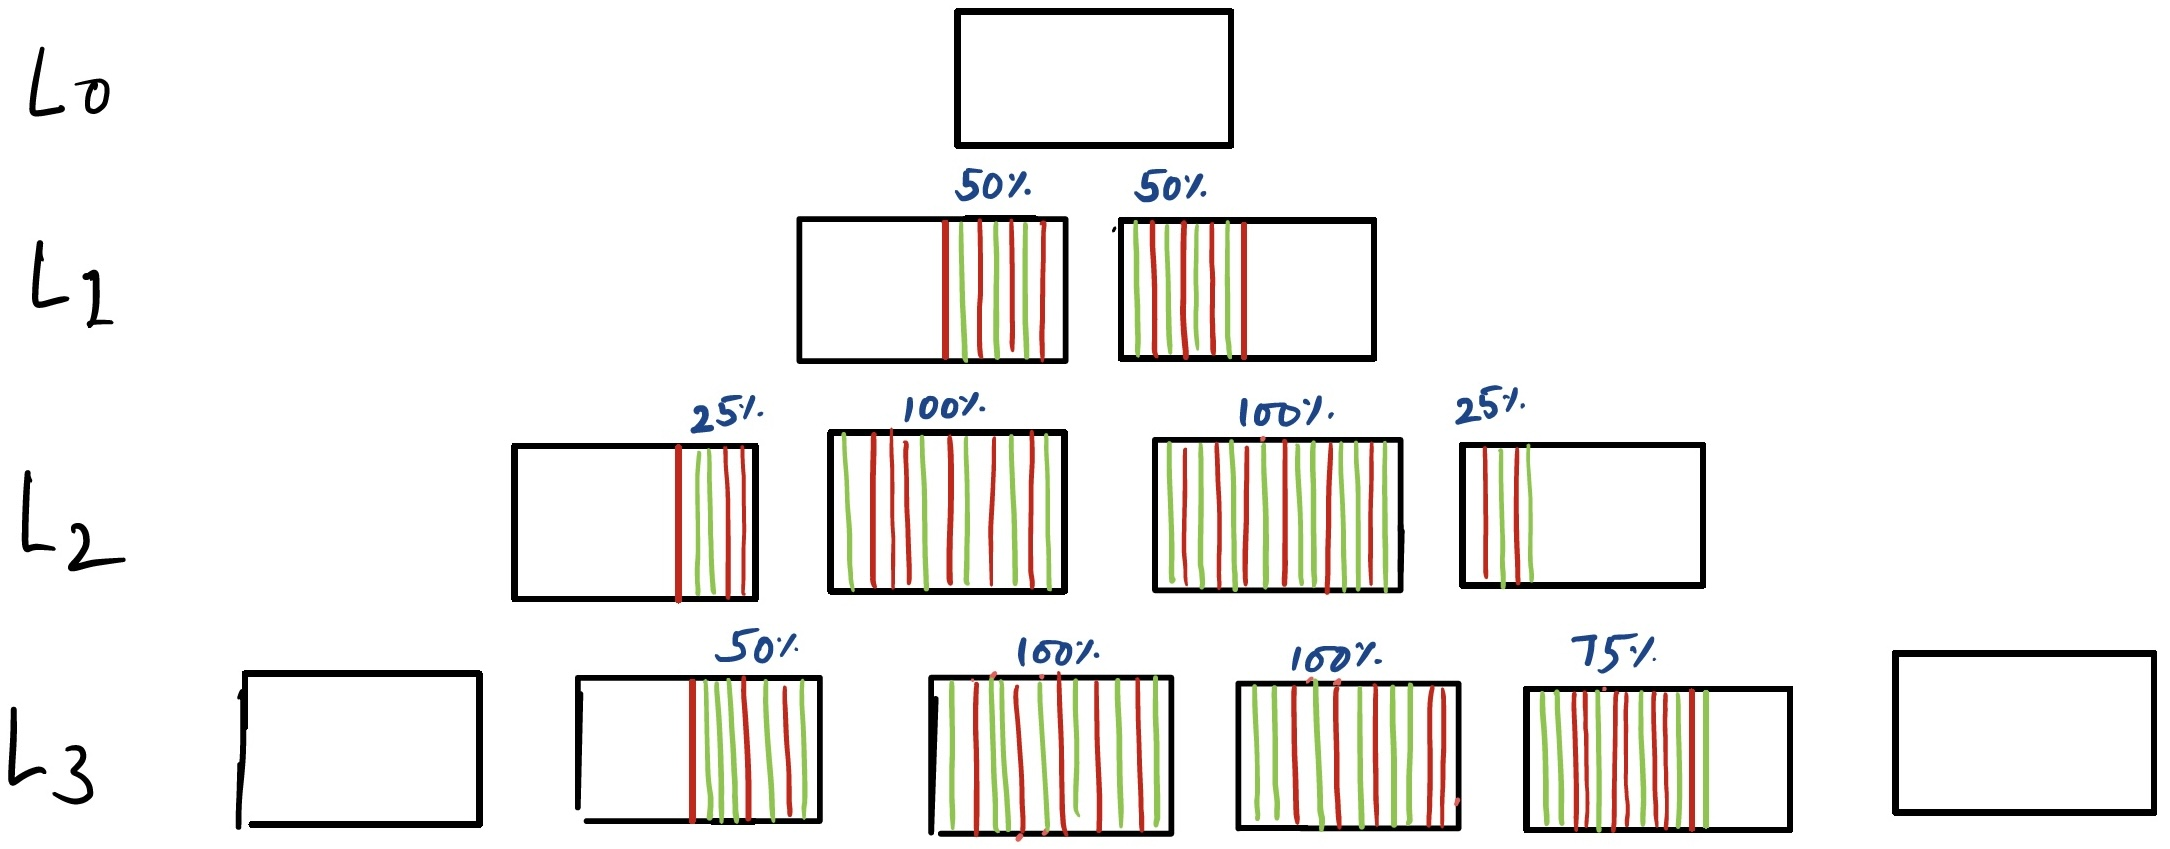
\includegraphics[scale=0.2]{Figures/first-state-lsm.jpg}
    \caption{Example demonstrating the query-driven compaction in a four-level LSM tree. The 
    LSM configuration includes a \textit{size ratio} of 2 \(T\), a page size of approximately 4 KB, a file size of around 
    2 MB, and 4 levels in the current state.}\label{fig:first-state-lsm}
\end{figure}

Let's try to understand this with an example. Consider we have an LSM with a \textit{size ratio} of 2 (T), a number
of pages of 512 (P), a number of entries per page of 4 (B), and an entry size of 1024 B (E). Assume we have 4 levels in 
the current LSM state (see Figure~\ref{fig:first-state-lsm}).

\begin{itemize}
    \item Page size $\colon B * E \approx 4 KB$
    \item File size $\colon P * B * E \approx 2 MB$
    \item Total entries in a file $\colon P * B \approx 2 K$
    \item $lower\_bound \colon 0.4\ \&\ upper\_bound \colon 1$ 
\end{itemize}

All the levels up to L2 are full, and L3 has 6 files. This means we have approximately 4K entries in L1 (2 SSTs), 8K in 
L2 (4 SSTs), and 12K in L3 (6 SSTs) as shown in Figure~\ref{fig:first-state-lsm}.

\begin{table*}
    \centering
    \begin{tabular}{ccc}

        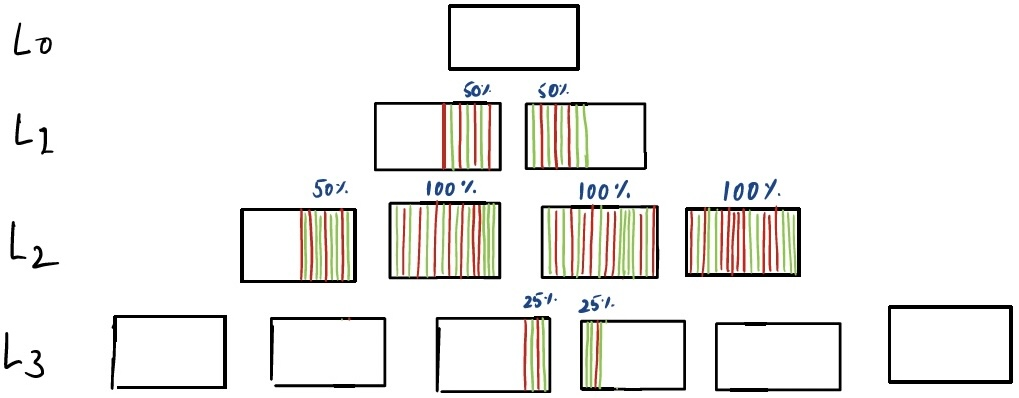
\includegraphics[scale=0.30]{Figures/fail-lsm-1.jpg} & 
        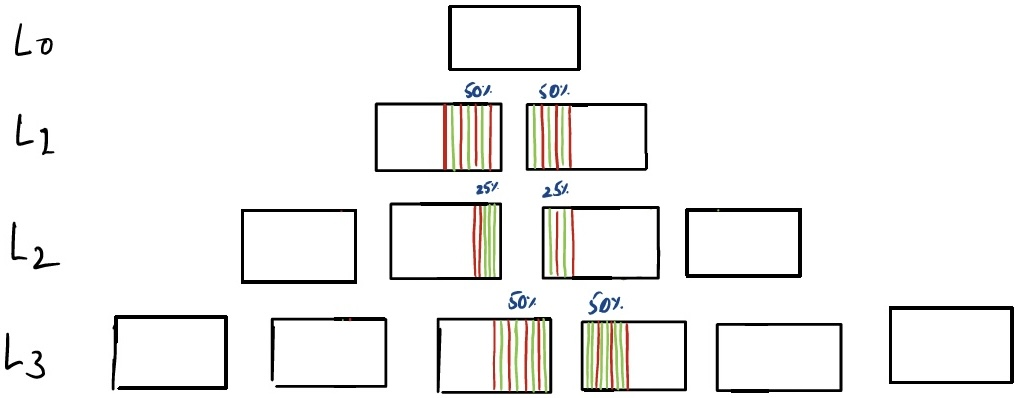
\includegraphics[scale=0.30]{Figures/fail-lsm-2.jpg} & 
        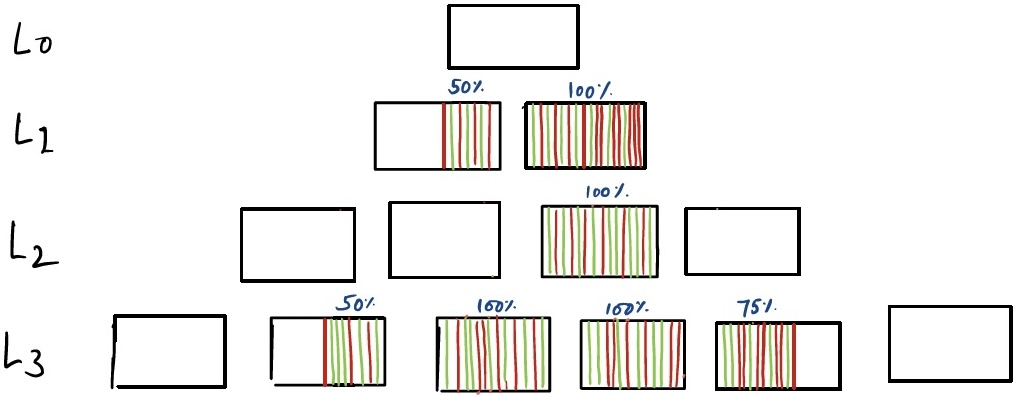
\includegraphics[scale=0.30]{Figures/fail-lsm-3.jpg}  
        \vspace{0.5em}\\
    
        \resizebox{0.3\textwidth}{!}{%
        \begin{tabular}{ |c|c|c|c| }
            \hline
            \textbf{Level} & \textbf{L-1} & \hspace*{4.1mm}\textbf{L-2}\hspace*{4.1mm} & \hspace*{4.1mm}\textbf{L-3}\hspace*{4.1mm} \\
            \hline
            \textbf{L-1} & [-] = T & [-, 0.28] = F & [-, 0.28, 14] = F \\
            \hline
            \textbf{L-2} & $\times$ & [-] = T & [-, 14] = F \\
            \hline
            \textbf{L-3} &  $\times$ &  $\times$ & [-] = T \\
            \hline
        \end{tabular}}
        
        &

        \resizebox{0.3\textwidth}{!}{%
        \begin{tabular}{ |c|c|c|c| }
            \hline
            \textbf{Level} & \textbf{L-1} & \hspace*{4.1mm}\textbf{L-2}\hspace*{4.1mm} & \hspace*{4.1mm}\textbf{L-3}\hspace*{4.1mm} \\
            \hline
            \textbf{L-1} & [-] = T & [-, 2] = F & [-, 2, 0.5] = F \\
            \hline
            \textbf{L-2} & $\times$ & [-] = T & [-, 0.5] = T \\
            \hline
            \textbf{L-3} &  $\times$ &  $\times$ & [-] = T \\
            \hline
        \end{tabular}}

        &

        \resizebox{0.3\textwidth}{!}{%
        \begin{tabular}{ |c|c|c|c| }
            \hline
            \textbf{Level} & \textbf{L-1} & \hspace*{4.1mm}\textbf{L-2}\hspace*{4.1mm} & \hspace*{4.1mm}\textbf{L-3}\hspace*{4.1mm} \\
            \hline
            \textbf{L-1} & [-] = T & [-, 1.5] = F & [-, 1.5, 0.30] = F \\
            \hline
            \textbf{L-2} & $\times$ & [-] = T & [-, 0.30] = F \\
            \hline
            \textbf{L-3} &  $\times$ &  $\times$ & [-] = T \\
            \hline
        \end{tabular}}
    \end{tabular}
    \caption{Examples highlighting scenarios where query-driven compaction is not performed, based on the decision 
    matrix. These instances provide insights into the conditions under which the system opts for the conventional 
    compaction approach.}\label{fig:not_performing_query-driven_compaction}
    \label{table:ex-not-performing-compaction}
\end{table*}

\begin{table}
    % \resizebox{\linewidth}{!}{%
    \begin{tabular}{|c|c|}
        \hline
        \textbf{Level} & \textbf{Number of Entries} \\
        \hline
        L-0 & \-- \\
        \hline
        L-1 & 2K \\
        \hline
        L-2 & 5K \\
        \hline
        L-3 & 6.5K \\
        \hline
    \end{tabular}
    % }
    \caption{Illustration of the \textit{$E_{useful}$} entries count for each level in the LSM tree for
    the example presented in Figure~\ref{fig:first-state-lsm}}
    \label{table:ex-decision-making-meta-data}
\end{table}

\begin{table}
    % \captionsetup{justification=centering,margin=2cm}
    \begin{tabular}{ |c|c|c|c| }
        \hline
        \textbf{Level} & \textbf{L-1} & \hspace*{4.1mm}\textbf{L-2}\hspace*{4.1mm} & \hspace*{4.1mm}\textbf{L-3}\hspace*{4.1mm} \\
        \hline
        \textbf{L-1} & [-] = T & [-, 0.4] = T & [-, 0.4, 0.76] = T \\
        \hline
        \textbf{L-2} & $\times$ & [-] = T & [-, 0.76] = T \\
        \hline
        \textbf{L-3} &  $\times$ &  $\times$ & [-] = T \\
        \hline
    \end{tabular}
    \caption{Decision matrix generated from the data in Table~\ref{table:ex-decision-making-meta-data}. Helps in 
    decision-making process for compaction, providing insights into the selection of levels based on \textit{lb} and \textit{ub}.}
    \label{table:ex-decision-matrix}
\end{table}

Now, consider a range query that will read entries from L1, L2, and L3 (shaded portion in Figure~\ref{fig:first-state-lsm}).
The $E_{useful}$ for $L_1$ would be $2K$, as $50\%$ entries from both the SST files falls in the range of the range query.
Similarly, the $E_{useful}$ for $L_2$ and $L_3$ would be $5K$ and $6.5K$ respectively (shown in Table-\ref{table:ex-decision-making-meta-data}). 
The decision matrix can be formed based on Table-\ref{table:ex-decision-making-meta-data} (as shown in 
Table-\ref{table:ex-decision-matrix}). For simplicity, let's assume that the range of keys from every level uniformly 
overlaps with the range of keys on the next level. In query-driven compaction, the algorithm selects the first ``True''
entry starting from the rightmost column of the decision matrix. This strategy is employed to maximize compaction, 
specifically targeting the removal of more invalid entries. The removal of invalid entries helps reduce space 
amplification, ultimately leading to decreased write amplification and improved performance in range queries.
For the above example, it is $L_{13}$.

Table~\ref{table:ex-not-performing-compaction} presents several scenarios where query-driven compaction may become an 
overhead, leading to a fallback to the vanilla approach. This lightweight strategy, employed before executing a range 
query, provides flexibility for more granular compactions based on the overlap between levels.

For instance, if a range query involves reading data from the first five levels and the keys between $level-2$ to 
$level-4$ exhibit significant overlap, the query-driven compaction mechanism will intelligently select $level-2$, 
$level-3$, and $level-4$ to merge the overlapping keys from the specified range. The resulting compaction will write 
the valid keys back to $level-4$, optimizing the storage structure for improved performance in handling range queries.

% The ratio\(s\) ($R_{ij}$) for the number of useful entries in level $i$ to the number of useful entries in level $j$ (where $j=i+1$).
% \hfill
% \begin{center}
% \begin{math}
%     L_{[start\ end]}=\left\{
%       \begin{array}{ll}
%         R_{ij} = \frac{E_{useful(i)}}{E_{useful(j)}} \quad \forall\ i=start\ to\ end,\ j=i+1\\
%         R_{ij} \geq lower\_bound\ \&\ R_{ij} \leq upper\_bound
%       \end{array}
%     \right.
%   \end{math}
% \end{center}
% \hfill \break